\begin{name}
	{ÔN TẬP KIỂM TRA GIỮA HỌC KÌ 1}
	{TOÁN 10}
	{LỚP TOÁN THẦY PHÁT}
	{\thoigian}
\end{name}

\caulc

\Opensolutionfile{ans}[ans-ABCD]

\begin{ex}%[0D1N1-1]%[CTST - Lớp 10 - Ôn tập giữa học kì 1 - Đề 2]%[Khổng Xuân Thạnh]
	Phát biểu nào sau đây là một mệnh đề toán học? 
	\choice
	{Thời tiết hôm nay lạnh quá!}
	{Đề thi môn Toán quá khó}
	{\True Hình bình hành có hai cặp cạnh bằng nhau}
	{Số $-3$ có phải là số tự nhiên không?}
	\loigiai
	{ Hình bình hành có hai cặp cạnh bằng nhau là một mệnh đề toán học.
	}
\end{ex}

\begin{ex}%[0D1N1-1]%[CTST - Lớp 10 - Ôn tập giữa học kì 1 - Đề 2]%[Khổng Xuân Thạnh]
	Trong các câu sau, câu nào \textbf{không} là mệnh đề chứa biến? 
	\choice
	{\True Số $2$ không phải là số nguyên tố}
	{$4x^2-x-5=0$}
	{$5x-2y=0$}
	{$2m+1$ chia hết cho $3$}
	\loigiai
	{Số $2$ không phải là số nguyên tố không phải là mệnh đề chứa biến.
	}
\end{ex}

\begin{ex}%[0D1H1-5]%[CTST - Lớp 10 - Ôn tập giữa học kì 1 - Đề 2]%[Khổng Xuân Thạnh]
	Trong các mệnh đề dưới đây, mệnh đề nào là mệnh đề đúng?  
	\choice
	{$\exists x \in \mathbb{R} \colon x^2+1=0$}
	{$\exists x \in \mathbb{R} \colon x^2<0$}
	{\True $\exists x \in \mathbb{N} \colon 2x^2-1<0$}
	{$\exists x \in \mathbb{N} \colon x^2-2=0$}
	\loigiai
	{
		\begin{itemize}
			\item Ta có $x^2 \geq 0 \Leftrightarrow x^2 +1 \geq 1$, $\forall x \in \mathbb{R}$. Vậy loại.
			\item Ta có $x^2 \geq 0$, $\forall x \in \mathbb{R}$. Vậy loại.
			\item $2x^2-1<0 \Leftrightarrow x^2<\dfrac{1}{2} \Leftrightarrow -\dfrac{\sqrt{2}}{2}<x<\dfrac{\sqrt{2}}{2}$, mà $x \in \mathbb{N}$ suy ra $x=0$. Vậy đúng.
			\item $x^2 -2=0 \Leftrightarrow x=\pm \sqrt{2} \notin \mathbb{N}$. Vậy loại.
		\end{itemize}
	}
\end{ex}

\begin{ex}%[0D1H2-1]%[CTST - Lớp 10 - Ôn tập giữa học kì 1 - Đề 2]%[Khổng Xuân Thạnh]
	Hãy liệt kê các phần tử của tập hợp $\mathrm{X}=\left\{x \in \mathbb{R}|x^2+x+1=0\right\}$.
	\choice
	{$\mathrm{X}=0$}
	{$\mathrm{X}=\{0\}$}
	{\True $\mathrm{X}=\varnothing$}
	{$\mathrm{X}=\{\varnothing\}$}
	\loigiai
	{
		Phương trình $x^2+x+1=0$ vô nghiệm nên $\mathrm{X}=\varnothing$.
	}
\end{ex}

\begin{ex}%[0D1H1-5]%[CTST - Lớp 10 - Ôn tập giữa học kì 1 - Đề 2]%[Khổng Xuân Thạnh]
	Cho các tập hợp $A=\left\{x \in \mathbb{N^*}|-4\leq 2x-1\leq 12\right\}$ và $B=[2;5)$. Tập hợp $A\setminus B$ có bao nhiêu phần tử?
	\choice
	{Vô số}
	{$1$}
	{$2$}
	{\True $3$}
	\loigiai
	{
		Ta có $-4 \leq 2x-1 \leq 12 \Leftrightarrow -\dfrac{3}{2} \leq x \leq \dfrac{13}{2}$.\\
		Do $x \in \mathbb{N^*}$ nên $A=\{1;2;3;4;5;6\}$ suy ra $A\setminus B=\{1;5;6\}$.\\
		Vậy $A\setminus B$ có $3$ phần tử.
	}
\end{ex}

\begin{ex}%[0D2H1-1]%[CTST - Lớp 10 - Ôn tập giữa học kì 1 - Đề 2]%[Khổng Xuân Thạnh]
	Cặp số $(2;-1)$ là nghiệm của bất phương trình nào dưới đây?
	\choice
	{$x+y-1<0$}
	{$2x+3y>1$}
	{$x+3y \geq 0$}
	{\True $x+2y \leq 0$}
	\loigiai
	{
		Lần lượt thay $x=2$; $y=-1$ vào các bất phương trình $x+2y \leq 0$ thấy thỏa mãn. 
	}
\end{ex}

\begin{ex}%[0D2H1-2]%[CTST - Lớp 10 - Ôn tập giữa học kì 1 - Đề 2]%[Khổng Xuân Thạnh]
	\immini{	Nửa mặt phẳng kể cả bờ (phần không bị gạch) trong hình vẽ dưới đây là miền nghiệm của bất 
		phương trình nào? \\
		\choice
		{\True $2x+y\geq 2$}
		{$2x+y\leq 2$}
		{$2x-y\geq 2$}
		{$2x-y\leq 2$}
	}{	\begin{tikzpicture}[>=stealth,line join=round,line cap=round,font=\footnotesize,scale=.4,x=1cm,y=1cm]
			\def\xmin{-4} \def\xmax{4}
			\def\ymin{-4} \def\ymax{5} 
			\draw[->] (\xmin,0)--(\xmax,0) node [above left]{$x$};
			\draw[->] (0,\ymin)--(0,\ymax) node [above right]{$y$};
			\foreach \x in {-3,-2,-1,1,2,3} {\draw (\x,0) node[below] {\scriptsize$\x$} circle (1pt);}
			\foreach \y in {-3,-2,-1,1,2,3,4} {\draw (0,\y) node[left] {\scriptsize$\y$} circle (1pt);} 
			\draw (0,0) node [below left, shift={(0.1,0.1)}]{\scriptsize$O$};	
			\clip (\xmin,\ymin) rectangle (\xmax,\ymax);
			\fill[pattern = north west lines,pattern color = black!70, smooth,opacity=0.5] 
			(\xmax,\ymin)--(\xmin,\ymin)--(\xmin,\ymax)--plot[domain= \xmin:\xmax](\x,{2-2*\x})-- cycle;
			\draw[color=black,line width=.5, smooth, samples=100, domain= -10:110] plot(\x,{2-2*\x});
	\end{tikzpicture}}
	\loigiai
	{
			Ta thấy bờ của nửa mặt phẳng đã cho là đường thẳng $d$ cắt các trục tọa độ tại $A(0;2)$, $B(1;0)$ nên $d$ có phương trình $y=-2x+2 \Leftrightarrow 2x+y=2$.\\
			Vì điểm $O(0;0)$ không phụ thuộc miền nghiệm của bất phương trình nên bất phương trình cần tìm là $2x+y\geq 2$.
	}
\end{ex}

\begin{ex}%[0D2H2-1]%[CTST - Lớp 10 - Ôn tập giữa học kì 1 - Đề 2]%[Khổng Xuân Thạnh]
	Cặp số nào dưới đây không là nghiệm của hệ bất phương trình $\heva{&x+2y>3 \\& 2x-y\leq 1}$?
	\choice
	{$(0;2)$}
	{$(1;2)$}
	{\True $(1;1)$}
	{$(-1;3)$}
	\loigiai
	{
		Thay lần lượt các cặp số trong các đáp án vào hệ ta thấy chỉ có cặp số $(1;1)$ không thỏa mãn hệ. 
	}
\end{ex}

\begin{ex}%[0H4N1-2]%[CTST - Lớp 10 - Ôn tập giữa học kì 1 - Đề 2]%[Khổng Xuân Thạnh]
	Chọn đáp án đúng. 
	\choice
	{$\sin 135^{\circ}=-\dfrac{\sqrt{2}}{2}$}
	{$\cos 45^{\circ}=-\dfrac{\sqrt{2}}{2}$}
	{$\tan 135^{\circ}=1$}
	{\True $\cot 135^{\circ}=-1$}
	\loigiai
	{
		Ta có $\cot 135^{\circ}=-1$.
	}
\end{ex}

\begin{ex}%[0H4N1-3]%[CTST - Lớp 10 - Ôn tập giữa học kì 1 - Đề 2]%[Khổng Xuân Thạnh]
	Tính giá trị của biểu thức $A=\sin (10^{\circ}) \cdot \sin (20^{\circ}) \ldots \sin (190^{\circ}) \cdot \sin (200^{\circ})$.
	\choice
	{$4$}
	{$2$}
	{\True $0$}
	{$-2$}
	\loigiai
	{
		Ta thấy trong tích có $\sin 180^{\circ}=0$ và do đó $A=0$.
	}
\end{ex}

\begin{ex}%[0H4N2-2]%[CTST - Lớp 10 - Ôn tập giữa học kì 1 - Đề 2]%[Khổng Xuân Thạnh]
	Cho tam giác $ABC$ có $AB=3$, $AC=7$, $BC=8$. Tính diện tích tam giác $ABC$.
	\choice
	{$S=5\sqrt{3}$}
	{\True $S=6\sqrt{3}$}
	{$S=4\sqrt{3}$}
	{$S=3\sqrt{3}$}
	\loigiai
	{
		Áp dụng công thức Hê - rông ta có $S=\sqrt{p(p-a)(p-b)(p-c)}=6\sqrt{3}$.
	}
\end{ex}

\begin{ex}% [0H4H1-3]%[CTST - Lớp 10 - Ôn tập giữa học kì 1 - Đề 2]%[Khổng Xuân Thạnh]
	Cho $\triangle ABC$, hệ thức nào sau đây đúng?
	\choice
	{$\sin (A+B)=\cos C$}
	{$\cos \left(\dfrac{A}{3}\right)=\sin \left(\dfrac{B+C}{3}\right)$}
	{$\sin (A+B+C)=1$}
	{\True $\cos \left(\dfrac{A}{2}\right)=\sin \left(\dfrac{B+C}{2}\right)$}
	\loigiai
	{
		Ta có $\sin \left(\dfrac{B+C}{2}\right)=\sin \left(\dfrac{180-A}{2}\right)=\sin \left( 90^{\circ}-\dfrac{A}{2}\right)=\cos \left(\dfrac{A}{2}\right)$.
	}
\end{ex}
\Closesolutionfile{ans}

% \indapan{6}{ans-ABCD}

\cauds

\Opensolutionfile{ans}[ans-DS]

\begin{ex}%[ID6]%[Tên sách - Lớp 1x - Ôn tập giữa học kì 1 - Đề y]%[Tên giáo viên soạn]
	Cho tập hợp $A=\left\{x\in\mathbb{N}|x\leq 3\right\}$; $B=\left\{x\in \mathbb{Z}|-3<x+1\leq 4\right\}$;\\
	$C=\left\{x\in \mathbb{R}|-3\leq 2x-1<7\right\}$.
	\choiceTF
	{$B=(-4;3]$}
	{\True $A\cup B=B$}
	{$(B\setminus A)\cap C=\{-1;4\}$}
	{\True $(A\setminus B)\subset B$}
	\loigiai
	{
		% Lời giải chung
		\begin{itemchoice}
			\itemch Sai. \\
			Ta có $-3<x+1\leq 4 \Leftrightarrow -4 <x\leq 3$, mà $x \in\mathbb{Z}$ nên $B=\{-3;-2;-1;0;1;2;3;4\}$. Suy ra mệnh đề sai.
			\itemch Đúng.\\
			$A=\{0;1;2;3\}$. Từ đó, $A \subset B$. Suy ra $A\cup B=B$. Suy ra mệnh đề đúng.
			\itemch Sai.\\
			$ B\setminus A=\{-3;-2;-1;4\}$;\\
			Vì $-3\leq 2x-1<7 \Leftrightarrow -1\leq x<4$; $x\in \mathbb{R}$ suy ra $C=[-1;4)$ nên $(B\setminus A)\cap C=\{-1\}$\\
			Suy ra mệnh đề sai.
			\itemch Đúng.\\
			Vì $A\subset C$ nên $\heva{&A\setminus C=\varnothing \\&\varnothing \subset B}$ suy ra $(A\setminus C) \subset B$. Suy ra mệnh đề đúng.
		\end{itemchoice}
	}
\end{ex}

\begin{ex}%[ID6]%[Tên sách - Lớp 1x - Ôn tập giữa học kì 1 - Đề y]%[Tên giáo viên soạn]
	Cho tam giác $ABC$ có $AB=2\,cm$, $AC=3\,cm$, $\widehat{BAC}=60^{\circ}$.
	\choiceTF
	{Độ dài cạnh $BC=7\,cm$}
	{$\sin \widehat{ABC}=\dfrac{3\sqrt{21}}{14}$}
	{Diện tích tam giác $ABC$ bằng $3\sqrt{3}$ (cm$^2$)}
	{Chiều cao $h$ hạ từ đỉnh $A$ của tam giác $ABC$ bằng $\dfrac{3\sqrt{3}}{7}$ (cm)}
	\loigiai
	{
		% Lời giải chung
		\begin{itemchoice}
			\itemch Sai. \\
			$BC^2=AB^2+AC^2-2\cdot AB\cdot AC\cdot \cos\widehat{BAC}=7$ (cm), suy ra $BC=\sqrt{7}$ (cm).\\ Vậy \textbf{a} sai.
			\itemch Đúng.\\
			$\dfrac{AC}{\sin B}=\dfrac{BC}{\sin A}$, suy ra $\sin B=\dfrac{AC\cdot \sin A}{BC}=\dfrac{3\cdot \sin 60^{\circ}}{\sqrt{7}}=\dfrac{3\sqrt{21}}{14}$. Vậy \textbf{b} đúng.
			\itemch Sai.\\
			$S_{\triangle ABC}=\dfrac{1}{2}\cdot AB\cdot AC\cdot \sin A=\dfrac{1}{2}\cdot 2\cdot 3\cdot \sin 60^{\circ}=\dfrac{3\sqrt{3}}{2}$ cm$^2$. Vậy \textbf{c} sai.
			\itemch Sai.\\
			Chiều cao $h$ hạ từ đỉnh $A$ của tam giác $ABC$ là $S_{\triangle ABC}=\dfrac{1}{2}\cdot BC\cdot h$,\\ suy ra $h=\dfrac{2\cdot S_{\triangle ABC}}{BC}=\dfrac{2\cdot \dfrac{3\sqrt{3}}{2}}{\sqrt{7}}=\dfrac{3\sqrt{21}}{7}$ (cm). Vậy \textbf{d} sai.
		\end{itemchoice}
	}
\end{ex}

\Closesolutionfile{ans}

\caukq
\begin{ex}%[2-MH-6-MH2025]%[VN-MT-3, Mã/Tên TV biên soạn]%[2D4H2-2]
	Cho các tập hợp $A=\left(2 ;+\infty\right)$ và $B=\left[m^{2}-7 ;+\infty\right)$ với $m>0$. Tìm số giá trị nguyên của $m$ để $A \setminus B$ là một khoảng $(a ; b)$ thoả mãn $b-a$ thuộc đoạn $[3 ; 16]$.
	\shortans[0]{$2$}
	\loigiai{
		Điều kiện để $A \setminus B \neq \varnothing$ là $\heva{&m^{2}-7>2 \\ &m>0} \Leftrightarrow\heva{&m^{2}>9 \\ &m>0} \Leftrightarrow m>3$.\\
		Khi đó $A \setminus B=\left(2 ; m^{2}-7\right) \Rightarrow a=2 ; b=m^{2}-7$.\\
		Ta có $b-a$ thuộc đoạn $[3 ; 16] \Leftrightarrow 3 \leq m^{2}-9 \leq 16 \Leftrightarrow 12 \leq m^{2} \leq 25$.\\
		Do $m>3$ và $m \in \mathbb{Z}$ nên $m \in\{4 ; 5\}$. Vậy có 2 giá trị $m$ nguyên thoả mãn.}
\end{ex}

\begin{ex}%[2-MH-6-MH2025]%[VN-MT-3, Mã/Tên TV biên soạn]%[2H5H2-8]
	Hình bình hành có hai cạnh là $5$ và $9$, một đường chéo bằng $11$. Tìm độ dài đường chéo còn lại (làm tròn đến một chữ số thập phân sau dấu phấy).
	\shortans{$9{,}5$}
	\loigiai{
		\begin{center}
			\begin{tikzpicture}
				
				% Xác định các điểm của hình bình hành
				\coordinate (A) at (0, 0);   % Điểm A
				\coordinate (B) at (5, 0);   % Cạnh AB có độ dài 5
				\coordinate (D) at (2, 4);   % Cạnh AD có độ dài 9
				\coordinate (C) at ($(B) + (D) - (A)$); % Điểm C sao cho ABCD là hình bình hành
				
				% Vẽ các cạnh của hình bình hành
				\draw[thick] (A) -- (B) -- (C) -- (D) -- cycle;
				
				% Vẽ các đường chéo AC và BD
				\draw[dashed] (A) -- (C);   % Đường chéo AC
				\draw[dashed] (B) -- (D);   % Đường chéo BD có độ dài 11
				
				% Gắn nhãn các đỉnh
				\node[below left] at (A) {$A$};
				\node[below right] at (B) {$B$};
				\node[above right] at (C) {$C$};
				\node[above left] at (D) {$D$};
				
				% Gắn nhãn các cạnh
				\node[below] at ($(A)!0.5!(B)$) {$9$};
				\node[left] at ($(A)!0.5!(D)$) {$5$};
				\node[above] at ($(A)!0.65!(C)$) {$11$};
				
			\end{tikzpicture}
		\end{center}
		Gọi hình bình hành là $ABCD$, $AD=5$, $AB=9$.\\
		Gọi $\alpha$ là góc đối diện với đường chéo có độ dài $11$.\\
		Ta có $\cos \alpha=\dfrac{5^2+9^2-11^2}{2\cdot 5\cdot 9}=-\dfrac{1}{6}$\\
		$\Rightarrow \alpha$ là góc tù $\Rightarrow \alpha=\widehat{BAD} \Rightarrow BD=11$\\
		$\Rightarrow AC^2=AD^2+DC^2-2 \cdot AD \cdot DC \cdot \cos \widehat{ADC}=AD^2+DC^2+2\cdot AD \cdot DC \cdot \cos \widehat{BAD}$\\
		(vì $\widehat{BAD}$ và $\widehat{ADC}$ bù nhau $\Rightarrow \cos \widehat{ADC}=-\cos \widehat{BAD}$)\\
		$\Rightarrow AC^2=5^2+9^2+2\cdot 5 \cdot 9 \cdot\left(-\dfrac{1}{6}\right)=91 \Rightarrow AC=\sqrt{91} \approx 9{,}5$.}
\end{ex}


\begin{ex}%[2-MH-6-MH2025]%[VN-MT-3, Mã/Tên TV biên soạn]%[2D1H5-8]
	Cho $\sin x+\cos x=\dfrac{2}{3}$, tính giá trị của biểu thức $P=\sin^3x+\cos^3x+\sin x \cos x$ (Kết quả làm tròn đến hai chữ số sau dấu phẩy).
	
	\shortans[]{$0{,}57$}
	\loigiai{Ta có $\sin x+\cos x=\dfrac{2}{3} \Rightarrow (\sin x+\cos x)^{2}=\dfrac{4}{9} \Leftrightarrow \sin^2 x+\cos^2 x+2\sin x \cos x=\dfrac{4}{9}$\\
		$\Leftrightarrow 2\sin x \cos x=-\dfrac{5}{9} \Rightarrow \sin x \cos x=-\dfrac{5}{18}$.\\
		Ta có $P=(\sin x+\cos x)^3-3\sin x \cos x(\sin x+\cos x)+\sin x \cos x=\dfrac{23}{27}-\dfrac{5}{18}=\dfrac{31}{54} \approx 0{,}57$.
	}
\end{ex}
\begin{ex}%[De-chuan-hoa-so-1]%[Diamond]%[0H4V2-1]
Cho tam giác $ABC$ có $\widehat{A}+\widehat{B}=135^{\circ} $; $A B=2$. Bán kính đường tròn ngoại tiếp tam giác $ABC$ (làm tròn đến hàng phần trăm) là
\shortans[]{$1{,}41$}
\loigiai{
Ta có $\widehat{C} = 180^\circ- \widehat{A}-\widehat{B} = 45^{\circ}$. \\
Áp dụng định lí sin ta có $R= \dfrac{AB}{2\sin C} = \dfrac{2}{2\sin 45^\circ} = \sqrt{2}\approx 1{,}41$.
}
\end{ex}
\Closesolutionfile{ans}
% \indapan{6}{ans-KQ}
\TL
\begin{ex}%[2-MH-6-MH2025]%[VN-MT-3, Mã/Tên TV biên soạn]%[1H8V7-9]
	Lớp 10D có $15$ học sinh giỏi Toán, $18$ học sinh giỏi Anh, $20$ học sinh giỏi Văn, $6$ học sinh giỏi cả Toán và Văn, $10$ học sinh giỏi cả Toán và Anh, $7$ học sinh giỏi cả Văn và Anh, $3$ học sinh giỏi cả ba môn Toán, Văn, Anh. Số học sinh lớp 10D là bao nhiêu?
	\loigiai{\begin{center}
			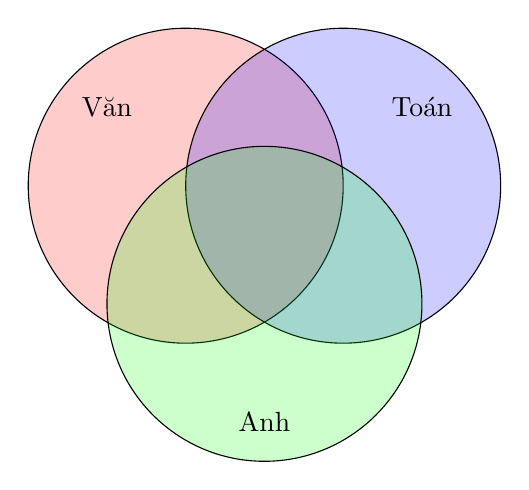
\begin{tikzpicture}
				% Set styles
				\tikzset{venn circle/.style={draw, circle, minimum width=4cm, fill opacity=0.2}}
				
				% Draw the three sets
				\node [venn circle, fill=red] (A) at (0,0) {};
				\node [venn circle, fill=blue] (B) at (2,0) {};
				\node [venn circle, fill=green] (C) at (1,-1.5) {};
				
				% Labels for the sets
				\node at (-1,1) {Văn};
				\node at (3,1) {Toán};
				\node at (1,-3) {Anh};
				
				% Overlapping areas (optional, depends on desired content)
				\node at (0.5,0.5) {}; % Overlap between Văn, Toán, Anh
				
			\end{tikzpicture}
		\end{center}
		Từ sơ đồ Ven ta có:\\
		Số học sinh chỉ giỏi Văn và Toán là: $6-3=3$ (học sinh).\\
		Số học sinh chỉ giỏi Văn và Anh là: $7-3=4$ (học sinh).\\
		Số học sinh chỉ giỏi Toán và Anh là: $10-3=7$ (học sinh).\\
		Khi đó ta có:\\
		Số học sinh chỉ giỏi Toán là: $15-3-3-7=2$ (học sinh).\\
		Số học sinh chỉ giỏi Văn là: $20-3-3-4=10$ (học sinh).\\
		Số học sinh chỉ giỏi Anh là: $18-3-4-7=4$ (học sinh).\\
		Vậy tổng số học sinh lớp 10D là: $3+(3+4+7)+(2+10+4)=33$ (học sinh).}
\end{ex}


\begin{ex}%[2-MH-6-MH2025]%[VN-MT-3, Mã/Tên TV biên soạn]%[2D6V1-2]
	Một bãi giữ xe ban đêm dành cho ôtô có diện tích đậu xe là $150$ m$^2$ (không tính lối đi cho xe ra vào). Biết rằng, một xe du lịch cần diện tích $3$ m$^2$ mỗi chiếc và phải trả phí $40$ nghìn đồng mỗi đêm, một xe tải cần diện tích $5$ m$^2$ mỗi chiếc và phải trả phí $50$ nghìn đồng mỗi đêm. Nhân viên quản lí không thể phục vụ quá $40$ xe một đêm. Doanh thu cao nhất mỗi đêm mà chủ bãi xe thu được là bao nhiêu nghìn đồng.
	
	% \shortans{$1750$}
	\loigiai{Gọi $x$ là số xe du lịch và $y$ là số xe tải mà chủ bãi xe nên cho đậu một đêm.\\
		Ta có hệ bất phương trình: $\left\{\begin{array}{l}x+y \leq 40 \\ 3 x+5 y \leq 150 \\ x \geq 0 \\ y \geq 0\end{array}\right.$ $(I)$\\
		Miền tứ giác $O A B C$ là miền nghiệm của hệ bất phương trình $(I)$, với $O(0 ; 0)$, $A(0 ; 30)$, $B(25 ; 15)$, $C(40 ; 0)$.
		\begin{center}
			\begin{tikzpicture}[scale=1, font=\footnotesize, line join=round, line cap=round, >=stealth]
				\begin{scope}
					\clip (-1,-1) rectangle (5.5,5);
					\fill[opacity=.2,pattern=north east lines] (-2,6)--(6,6)--(6,-2)--cycle;
					\fill[opacity=.2,pattern=north west lines] (-4,5.4)--(7,5.4)--(7,-1.2)--cycle;
					\fill[opacity=.2,pattern=north east lines] (0,-1)--(-1,-1)--(-1,5)--(0,5)--cycle;
					\fill[opacity=.2,pattern=north west lines] (-1,0)--(-1,-1)--(5.5,-1)--(5.5,0)--cycle;
					\draw (-1,5)--(5,-1);
					\draw (-3.33,5)--(6.67,-1);
				\end{scope}
				\draw[->] (-1,0)--(5.5,0) node[below right]{$x$};
				\draw[->] (0,-1)--(0,5) node[above right]{$y$};
				\draw (1pt,3)--(-1pt,3) node[left]{$30$};
				\draw (1pt,4)--(-1pt,4) node[left]{$40$};
				\draw (4,1pt)--(4,-1pt) node[below]{$40$};
				\draw (5,1pt)--(5,-1pt) node[below]{$50$};
				\draw (2.5,1pt)--(2.5,-1pt) node[below]{$25$};
				\draw (1pt,1.5)--(-1pt,1.5) node[left]{$15$};
				\draw[dashed] (2.5,0)--(2.5,1.5)--(0,1.5);
				\draw[fill=black] (0,0) circle (1pt) node[below left]{$O$} (0,3) circle (1pt) node[above right]{$A$} (2.5,1.5) circle (1pt) node[above right]{$B$} (4,0) circle (1pt) node[above]{$C$};
			\end{tikzpicture}
		\end{center}
		Số tiền chủ bãi xe thu được $F(x;y)=40x+50y$ (nghìn đồng)\\
		Bào toán trở thành tìm giá trị lớn nhất của $F(x;y)$ với $F(x;y)$ thỏa mãn $(I)$.\\
		Ta có $F(0;0)=0$, $F(0;30)=1500$; $F(25 ; 15)=1750$; $F(40 ; 0)=1600$.\\
		Vậy doanh thu lớn nhất là $1750$ nghìn đồng tại điểm có tọa độ $(25 ; 15)$.
	}
\end{ex}

\begin{ex}%[De-chuan-hoa-so-13]%[Huỳnh Quy]%[0H4V2-2]
\immini{Anh Việt có một mảnh đất hình tứ giác $ABCD$ với $AB=4{,}2$ m, $BC=15{,}3$ m, $CD=5{,}4$ m, $DA=16{,}8$ m. Để tính diện tích mảnh đất, anh Việt lấy các điểm $M$, $N$ lần lượt trên các cạnh $AB$, $AD$ sao cho $AM=1$ m, $AN=1$ m. Anh Việt đo được $MN=1{,}7$ m. Tính diện tích mảnh đất (làm tròn kết quả đến hàng phần trăm).}{\begin{tikzpicture}[>=stealth,line join=round,line cap=round,font=\footnotesize,scale=.4]
\clip
(-2.2,-4)rectangle (18,6);
\path (0,0)coordinate (A)
++(90:4.2)coordinate (B)
++(0:15.3)coordinate (C)
;
\path[name path=c1] (C)circle(5.4)
;
\path[name path=c2] (A)circle(16.8)
;
\path[name intersections={of=c1 and c2}] (intersection-2) coordinate (D);
\draw
($(A)!1 cm!(B)$)coordinate (M)
--($(A)!1 cm!(D)$)coordinate (N)
(B)--(D)
(A)--(B)node[midway,left]{$4{,}2$ m}
(B)--(C)node[midway,above]{$15{,}3$ m}
(C)--(D)node[midway,right]{$5{,}4$ m}
(D)--(A)node[midway,below]{$16{,}8$ m}
;
\foreach \x/\g in {A/201,B/90,C/60,D/-90,M/180,N/-90} \fill (\x) circle (0.05)+(\g:.5) node{$\x$};
\end{tikzpicture}}
% \shortans[]{$64{,}59$}
\loigiai{
\begin{center}
\begin{tikzpicture}[>=stealth,line join=round,line cap=round,font=\footnotesize,scale=.6]
\clip
(-2,-4)rectangle (18,6);
\path (0,0)coordinate (A)
++(90:4.2)coordinate (B)
++(0:15.3)coordinate (C)
;
\path[name path=c1] (C)circle(5.4);
\path[name path=c2] (A)circle(16.8);
\path[name intersections={of=c1 and c2}] (intersection-2) coordinate (D);

\draw
($(A)!1 cm!(B)$)coordinate (M)
--($(A)!1 cm!(D)$)coordinate (N)
(B)--(D)
(A)--(B)node[midway,left]{$4{,}2$ m}
(B)--(C)node[midway,above]{$15{,}3$ m}
(C)--(D)node[midway,right]{$5{,}4$ m}
(D)--(A)node[midway,below]{$16{,}8$ m}
;
\foreach \x/\g in {A/201,B/90,C/60,D/-90,M/180,N/-90} \fill (\x) circle (0.05)+(\g:.5) node{$\x$};
\end{tikzpicture}
\end{center}
Xét tam giác $AMN$ có $AM=AN=1$ m, $MN=1{,}7$ m nên
\[\cos A=\dfrac{AM^2+AN^2-M^2}{2AM\cdot AN}=-0{,}445.\]
Suy ra
\[BD^2=AB^2+AD^2-2AB\cdot AD\cos A=4{,}2^2+16{,}8^2-2\cdot 4{,}2\cdot 16{,}8\cdot (-0{,}445)=362{,}6784\]
do đó, $BD=\sqrt{362{,}6784}$.\\
Áp dụng công thức Hê-rông ta có diện tích của  mảnh vườn tứ giác $ABCD$ là
\begin{eqnarray*}
S_{ABCD}&=&S_{ABD}+S_{BCD}\\&=&\dfrac{1}{4}\sqrt{(AB+BD+DA)(AB+BD-DA)(AB-BD+DA)(-AB+BD+DA)}\\
&	+&\dfrac{1}{4}\sqrt{(BC+CD+DB)(BC+CD-DB)(BC-CD+DB)(-BC+CD+DB)}\\
&\approx&64{,}59.
\end{eqnarray*}
}
\end{ex}
